\section{Training-Seed Sensitivity (LiteSSM-A and EfficientNet-B0)}
\label{app:seed}

Primary tables remain single-seed (training seed~42) with bootstrap CIs that quantify \emph{test-sample} uncertainty only.
To probe training-seed sensitivity under the locked Panel~A recipe (same manifests, 15~epochs, batch~64, AdamW $\mathrm{lr}=10^{-4}$), we additionally trained LiteSSM-A and EfficientNet-B0 with seeds~$\{43,44\}$ and re-evaluated ID test AUC and UFD Macro on the frozen UFD subset list.
Seed~42 reuses the released bake-off / baseline checkpoints.
Table~\ref{tab:seed-app} and Figure~\ref{fig:seed-app} report per-seed scores and population mean$\pm$std over the three runs.
LiteSSM-A Macro std remains small ($0.009$), consistent with stability under the locked recipe; EfficientNet-B0 Macro varies more ($0.022$), so we do \emph{not} replace primary rankings with these means.

\begin{figure}[H]
\centering
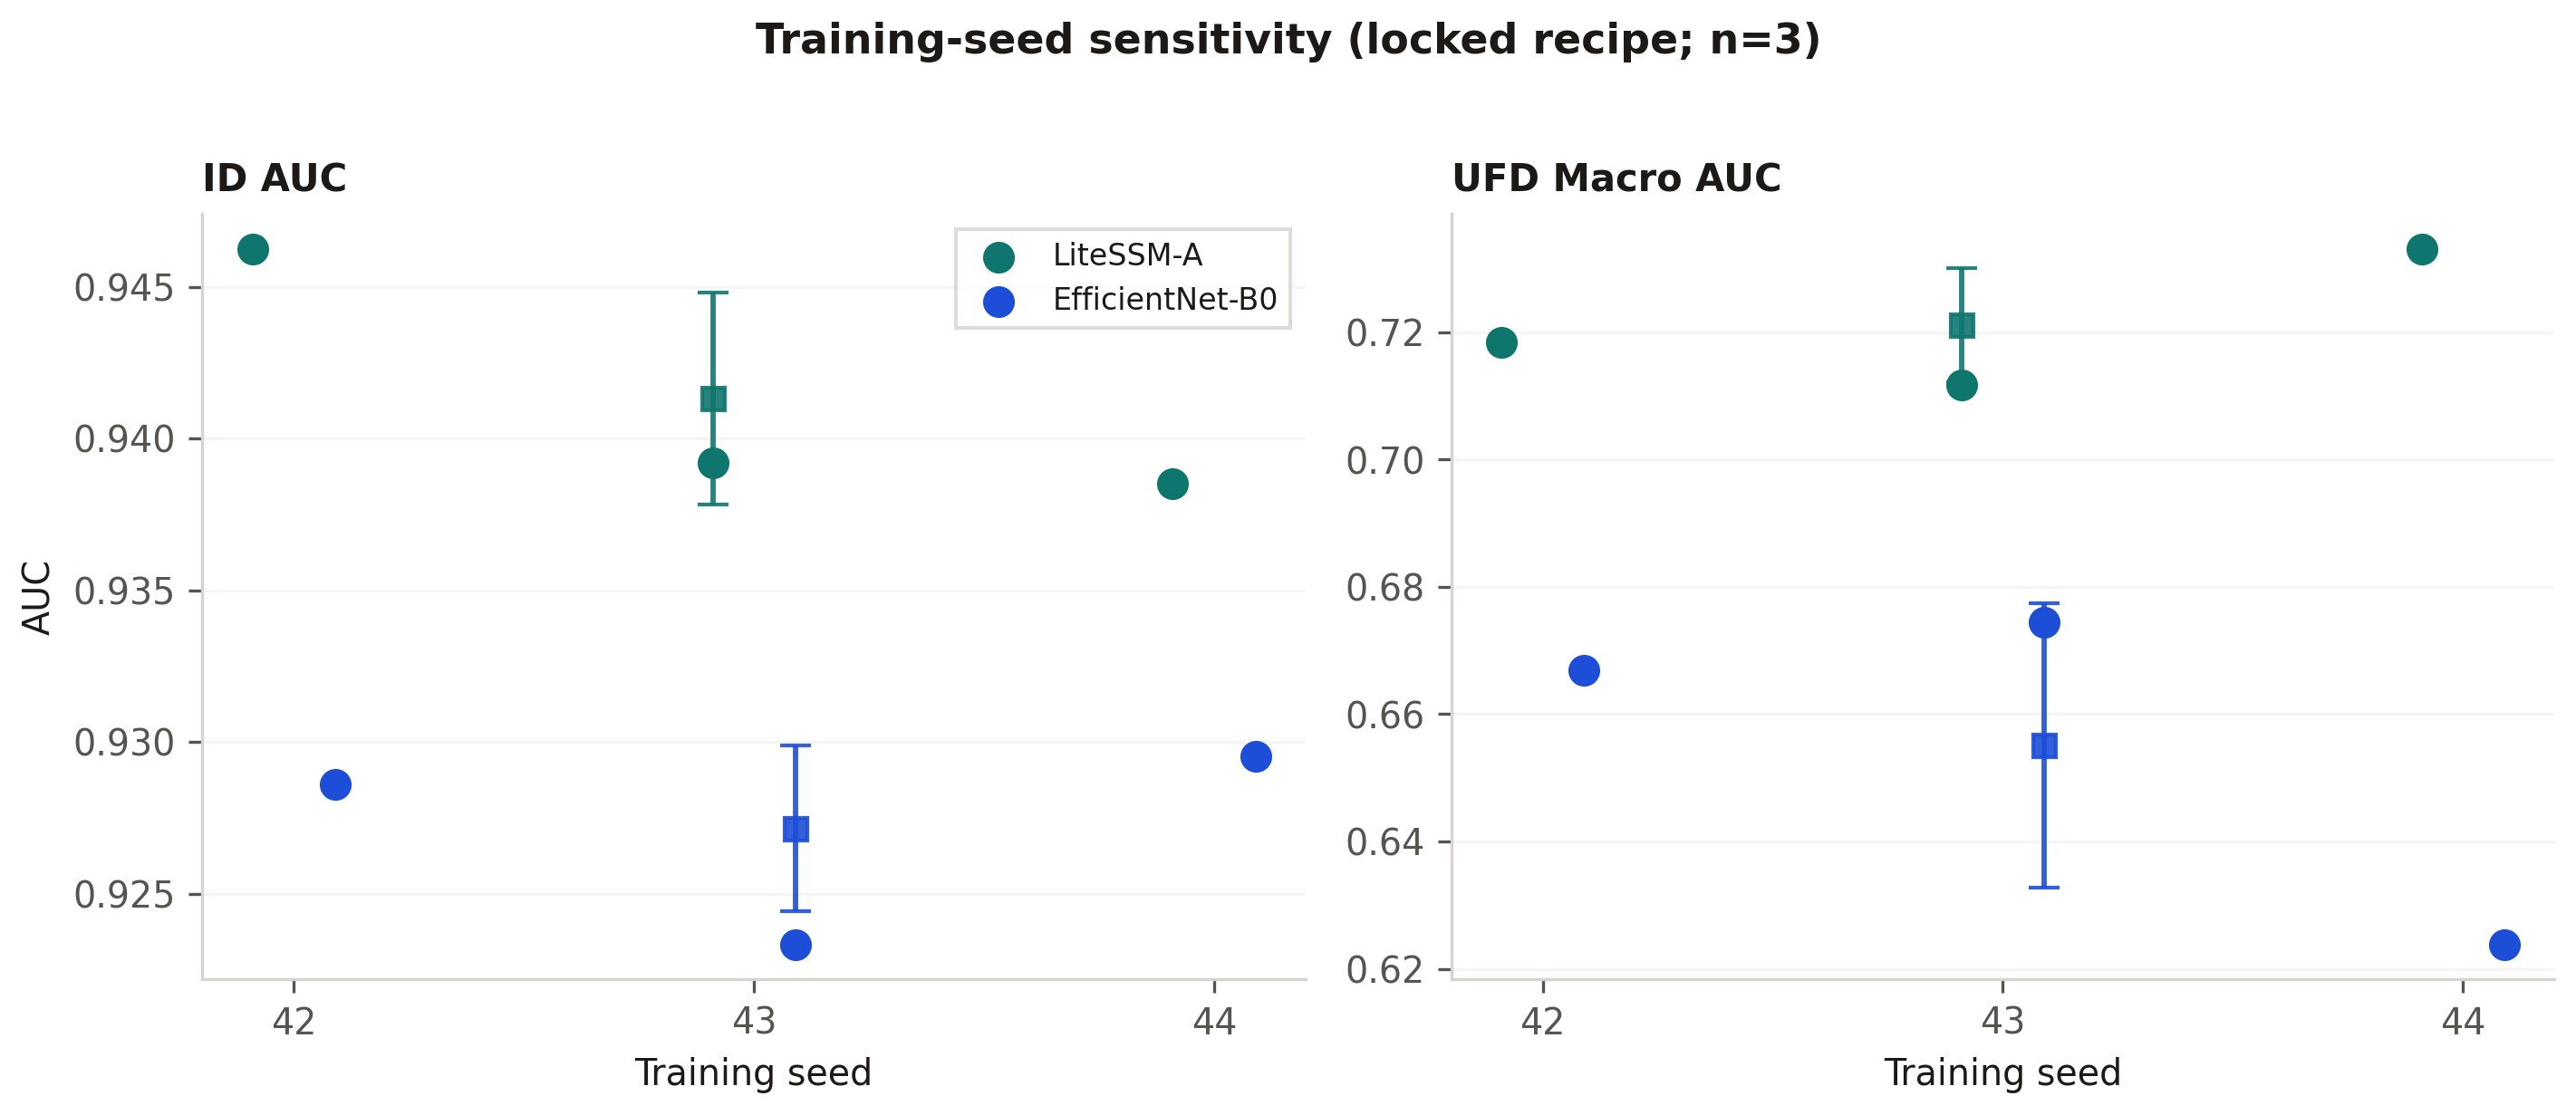
\includegraphics[width=0.95\textwidth]{figures/fig_seed_sensitivity.png}
\caption{Per-seed ID and UFD Macro AUC for LiteSSM-A and EfficientNet-B0 (seeds 42/43/44).
Squares show mean$\pm$population std.\label{fig:seed-app}}
\end{figure}

\begin{table}[H]
\caption{ID and UFD Macro AUC across training seeds 42/43/44 (locked recipe).\label{tab:seed-app}}
\begin{tabularx}{\textwidth}{l RRRRR}
\toprule
\textbf{Model} & \textbf{Metric} & \textbf{s42} & \textbf{s43} & \textbf{s44} & \textbf{Mean$\pm$std} \\
\midrule
LiteSSM-A & ID & 0.946 & 0.939 & 0.939 & $0.941\pm0.004$ \\
LiteSSM-A & UFD Macro & 0.718 & 0.712 & 0.733 & $0.721\pm0.009$ \\
EfficientNet-B0 & ID & 0.929 & 0.923 & 0.930 & $0.927\pm0.003$ \\
EfficientNet-B0 & UFD Macro & 0.667 & 0.674 & 0.624 & $0.655\pm0.022$ \\
\bottomrule
\end{tabularx}
\end{table}
